\newcommand{\acarbon}{$\alpha$-carbon}
\newcommand{\acarbons}{$\alpha$-carbons}
\newcommand{\invitro}{\textit{in vitro}}
\newcommand{\invivo}{\textit{in vivo}}
\newcommand{\ecoli}{\textit{E. coli}}

\chapter{Computational design of protein-based small molecule biosensors}


Living systems use naturally evolved sensors to detect the concentration of small molecules within cells.
Fluctuations in these concentrations often signal environmental change that must be met with tuned signaling responses, altering cell physiology and metabolism.
The ability to create new sensors for any small molecule would impact the study of many biological processes in cell and developmental biology through real time measurement of small molecule concentrations \invivo, serving as a valuable basic research tool.
Engineered biosensors could also tune biological processes dynamically in response to intracellular and external small molecule inputs, leading to applications in applied fields and medicine.
I propose to develop and test a computational design strategy to engineer such new biosensors.

\begin{figure}[H]
  \centering
  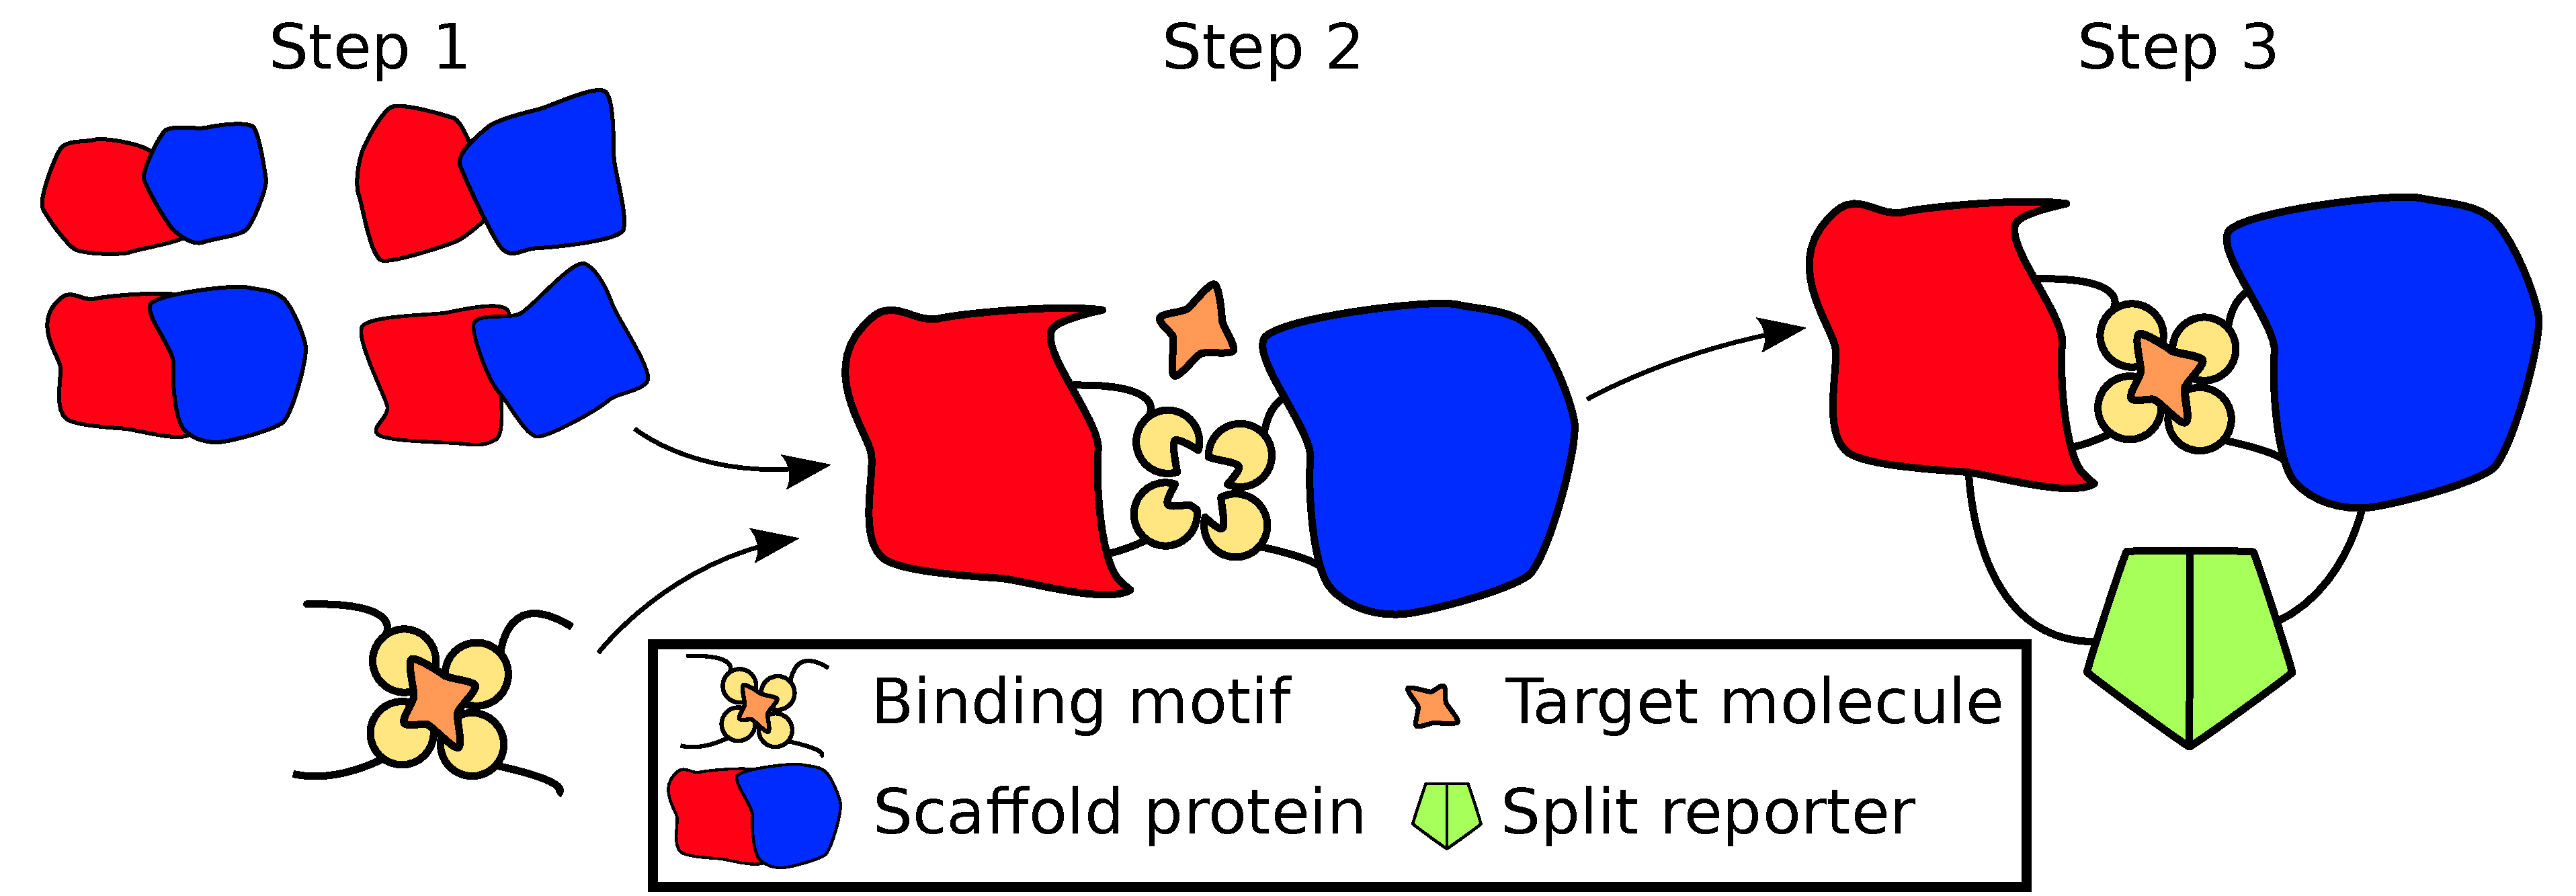
\includegraphics[width=\textwidth,keepaspectratio]{figures/biosensor-fig1-crop.pdf}
  \caption[Outline of the motif-directed computational design approach]{
    Outline of the motif-directed computational design approach.
    \textbf{Step 1:} Search for a heterodimeric protein-protein interface ``scaffold'' that can accommodate defined motif residues in the correct geometry to recognize a small molecule.
    %\thefontsize
    \textbf{Step 2:} Place the desired motif residues in dimer interface and design surrounding residues to accommodate the motif mutations.
    \textbf{Step 3:} Link a split reporter fragment (such as GFP or DHFR) to each half of the designed biosensor to sense the target by induced dimerization.
  }
  \label{fig:schematic-outline}
\end{figure}

I will engineer biosensors by adapting computational methods to redesign protein interfaces so that protein-protein association becomes dependent on small molecule presence (\cref{fig:schematic-outline}).
By linking the two protein partners to split reporters such as split green fluorescent protein (GFP), split enzymes, or two-hybrid activators, the target can then be detected in a modular fashion by optical, enzymatic or transcriptional readouts.
The design method I will develop takes known protein-protein interfaces as ``scaffolds'' into which a small molecule binding site can be placed, or ``matched''.
The binding site consists of a defined set of amino acids and their corresponding side chain conformations (``motif residues''), taken from a monomeric protein structure bound to the target small molecule.

\subsection{Significance}

Long-term, there are many significant applications of technologies to engineer new molecules that can sense currently undetectable molecules and can regulate biological behaviors in response.
One example is metabolic engineering, by controlling microbial pathways to maximize production of industrially valuable chemicals and fuels.
Another example is probing cell signaling, by controlling key protein-protein interactions with small-molecule induced dimerization.
I have chosen examples in each of the two areas.
In the first, I will develop sensors for farnesyl pyrophosphate (FPP), a central metabolic intermediate in pathways leading to biofuels, specialty chemicals and therapeutics\cite{zhang_metabolic_2011}.
In the second, I will engineer protein-protein interactions sensitive to inducers that do not have the undesired side effects of the currently used rapamycin-based system\cite{gray_activation_2010} (such as ergosterol, which does not occur in animals) or are triggered by small molecules that are light-switchable (such as p-coumaric acid), which would provide an additional layer of control.

\subsection{Accomplished research and remaining challenges}

A procedure to transplant defined motif residues into a protein scaffold has already been implemented in the design program Rosetta\cite{jiang_novo_2008} co-developed by the Kortemme lab.
We have adapted this method to biosensor engineering, and have demonstrated proof-of-concept for our strategy by generating sensor activity for FPP.

\newcommand{\matchingmotifcaption}{
  This model structure (colored) produced by computational design to bind FPP (pink) is not an exact match for the desired motif residue side chain positions (white).
  Aim 1 will test if more precise matches can be designed if the protein backbone is remodeled around ideally placed side chains.
}

\begin{figure}[H]
  \centering
  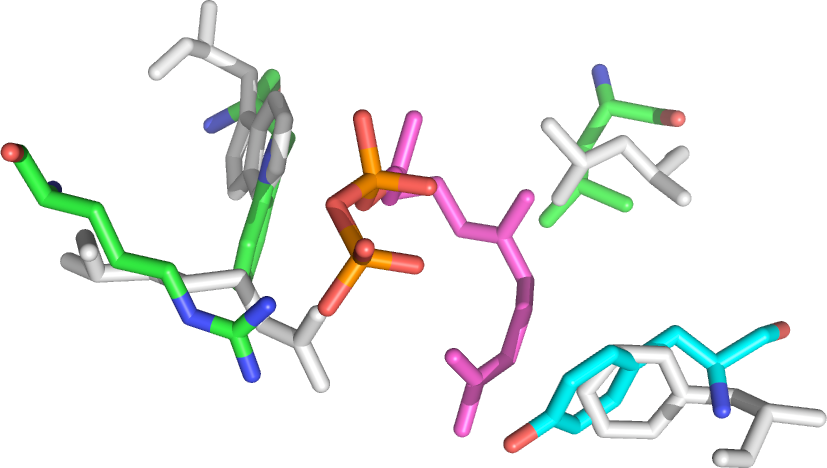
\includegraphics[width=\textwidth,keepaspectratio]{figures/biosensor-fig-2.png}
  \caption[Example of current matcher performance]{
    This model structure (colored) produced by computational design to bind FPP (pink) is not an exact match for the desired motif residue side chain positions (white).
    Aim 1 will test if more precise matches can be designed if the protein backbone is remodeled around ideally placed side chains.
  }
  \label{fig:matching-motif}
\end{figure}

Implementing side chain-centric backbone redesign within Rosetta allows me to implement a novel method for design while still taking advantage of the Rosetta energy function and proven design framework\cite{jiang_novo_2008}\cite{khersonsky_optimization_2011}.

\subsection{Aim 2: Engineer and optimize small molecule biosensors}

\noindent
\underline{Rationale}: Characterizing designed biosensors experimentally will provide data to feed back into the computational phase.
Because computational design is likely not accurate enough to predict which designed sequences will have the desired sensitivity, dynamic range, and specificity, I will experimentally test designed libraries (10-100 candidates) for initial activity.
This will take advantage of my engineering strategy (Fig.\ref{fig:schematic-outline}), where the sensor output can be used directly to assay the designs and subsequently improve starting activity by directed evolution.

\noindent
\underline{Approach}:
I will evaluate the generalizability of my approach by using a limited set of natural proteins as adaptable scaffolds to recognize multiple small molecule targets.
%% One promising scaffold is the FKBP/FRB complex.
%% As the rapamycin induced association of these proteins is a natural analogue of the biosensor design strategy, the rapamycin binding site within the FKBP/FRB complex is a promising candidate for designed recognition of other small molecules similar in size to rapamycin.
The computational improvements discussed in Aim 1 should, if successful, allow for scaffold protein dimers to accommodate a more diverse and complex set of small molecule targets due to the ensemble of backbone conformations generated during the matching protocol.
I can test this hypothesis directly by comparing the success of my modified matching and design protocol at supporting desired side chain geometries, compared to designs generated using the existing protocol.

I will design new sensors for several target small molecules.
These will include serotonin, a significant target in the study of neurobiology, and ibuprofen and ergosterol (a precursor to vitamin D$_2$\ found in fungi), which could function as generalized inducers of protein association to study signaling pathways.

Sensor output can be used to screen design candidates by using a split GFP reporter system where small molecule dependent dimerization induces fluorescence.
Split mammalian dihydrofolate reductase (DHFR) can also be used to select for active biosensors in \textit{E. coli}\ in the presence of the inhibitor thrimethoprim.
I will continue to use split GFP and DHFR linked biosensors for initial activity screens in cells.
For more detailed quantitative and structural characterization of successful designs, I will use isothermal titration calorimetry, NMR spectroscopy and X-ray crystallography.
These assays can be used to troubleshoot designs with weak activity by determining which half of the dimer pair most needs optimization to enhance ligand binding affinity, or alternatively, if destabilizing mutations need to be introduced to increase the free energy of association of the apo complex.

The activity and dynamic range of successful sensor designs can then be improved through directed evolution techniques.
My chances of success in Aim 2 can be improved by the new design method described in Aim 1, but success is not dependent on new methods, as sensors showing initial activity have already been developed in our lab for FPP.
